\documentclass[11pt,letterpaper]{article}
\usepackage[margin=1in]{geometry}
\usepackage[T1]{fontenc}
\usepackage{lmodern,amsmath,amssymb,amsthm,mathtools,microtype}
\usepackage{booktabs,longtable,array,graphicx,xcolor,enumitem,fancyhdr,listings}
\usepackage{xurl}
\usepackage{hyperref}
\definecolor{ink}{HTML}{14334A}
\definecolor{accent}{HTML}{137B80}
\hypersetup{colorlinks=true,linkcolor=ink,citecolor=accent,urlcolor=accent,
  pdftitle={Affine families and inherited structure in unknot recognition},
  pdfauthor={Research prepared for Vladimir Reshetnikov with ChatGPT}}
\setlength{\headheight}{15pt}
\pagestyle{fancy}\fancyhf{}
\fancyhead[L]{\small\color{ink}Affine families and inherited structure}
\fancyhead[R]{\small ProveIt research}
\fancyfoot[C]{\thepage}
\setlength{\parskip}{4pt}
\setlength{\parindent}{1.2em}
\setlist{itemsep=3pt,topsep=4pt}
\newtheorem{theorem}{Theorem}[section]
\newtheorem{lemma}[theorem]{Lemma}
\newtheorem{proposition}[theorem]{Proposition}
\newtheorem{corollary}[theorem]{Corollary}
\theoremstyle{definition}
\newtheorem{definition}[theorem]{Definition}
\newtheorem{example}[theorem]{Example}
\newtheorem{remark}[theorem]{Remark}
\newcommand{\Z}{\mathbb Z}
\newcommand{\F}{\mathbb F}
\newcommand{\Q}{\mathbb Q}
\newcommand{\R}{\mathbb R}
\newcommand{\End}{\operatorname{End}}
\newcommand{\im}{\operatorname{im}}
\newcommand{\rank}{\operatorname{rank}}
\newcommand{\poly}{\operatorname{poly}}
\newcommand{\code}[1]{{\small\nolinkurl{#1}}}
\newcommand{\sourcepin}{\texttt{ea9cf443c8ce}}
\lstset{basicstyle=\ttfamily\footnotesize,breaklines=true,columns=fullflexible,
  keepspaces=true,frame=single,rulecolor=\color{black!15},showstringspaces=false}
\title{\color{ink}\textbf{Affine Families and Inherited Structure\\in Unknot Recognition}\\[6pt]
  \large Certified component optimization, normal-coordinate extraction,\\
  and reuse of scalar endomorphism spaces}
\author{Research continuation prepared for Vladimir Reshetnikov\\
  \small ProveIt / Topology / UnknotRecognition\\
  \small Mathematical development, implementation, and independent model-assisted review}
\date{8 October 2026}
\begin{document}
\maketitle
\begin{abstract}
We continue the ProveIt unknot-recognition program at a pinned repository
revision. The main arithmetic result replaces enumeration by an exact
optimization over an entire affine family. For a binary modulus $m$, a
nonempty solution set $Az=b\pmod m$, and cyclic monodromies
$h(z)=c+Hz$, we determine
$\min_z\gcd(m,h_1(z),\ldots,h_r(z))$ in deterministic polynomial bit time.
The minimum is attained by a constructively produced assignment, without
integer factorization. Compact dual modular identities certify both
optimality and infeasibility independently of the optimizer. We connect
this result to full-boundary assemblies of cyclic surface covers, allowing
disconnected local covers and correlated seam parameters.

A second contribution extracts signed interval pairings and prism-gap
contacts directly from admissible binary normal coordinates in tetrahedra,
with a number of records linear in the triangulation size and independent
of the number of normal discs. A third implements inheritance of scalar
endomorphism spaces after verified chain-complex splitting, replacing
descendant commutator solves by restriction of a transported parent basis.
A dimension-saturated generator can additionally certify scalar locality
and permit inheritance through one generator. The article gives proofs, exact-input contracts, independent finite
checks, paired benchmarks, negative results, and a research agenda.
These results improve specific represented operations. They do not prove
a general quasi-polynomial unknot-recognition bound; global state growth,
geometric admissibility, and hierarchy restart costs remain explicit.
\end{abstract}
\clearpage
\tableofcontents
\clearpage
\section{The continuation and its exact scope}
\label{sec:scope}

\subsection{What problem is being improved?}

The long-term objective is a complete algorithm deciding whether a classical
knot diagram with $n$ crossings represents the unknot in time
$n^{O(\log n)}=2^{O((\log n)^2)}$. This is a statement about the entire
computation, including preprocessing, state construction, every restart,
coefficient bit lengths, and the final verdict. More generally,
quasi-polynomial means $\exp((\log(n+2))^{O(1)})$; we focus on the
concrete squared-logarithm target. A polynomial subroutine
for an exponentially large state is not sufficient.

The maintained implementation combines inexpensive certificates and
invariant filters with complete, potentially exponential fallback
algorithms. Its Khovanov route uses a tangles-and-cobordisms formulation
of chain complexes, following the framework of Bar-Natan~\cite{barnatan};
the unknot-detection theorem itself is due to Kronheimer and
Mrowka~\cite{km}. Exactness and the worst-case running time are separate
questions. In particular, a filter which has not detected an obstruction
has not proved the knot trivial.

This continuation audits the repository at \sourcepin, fetched on
8 October 2026. The initial remote inspection saw the immediately earlier
revision \code{04d799b69d38}; the branch advanced
while the sparse checkout was being obtained. All patches, baseline
comparisons, and distributed source hashes use the actual checked-out
revision \sourcepin. No inference is made from a mutable \code{main} URL
after that point. The full baseline identifier is:
\begin{center}
\code{ea9cf443c8ce33e09ed0c48b0ef7856ddf6326a3}
\end{center}

\subsection{The three bottlenecks addressed}

Recent incoming reports already supplied polynomial projectors, compressed
surface-cover assembly, regular-cover gluing equivalence, and a binary
normal-disc certificate checker~\cite{projectors,certificates}. We use
their precise scope, including their negative measurements. The present
work advances three subsequent tasks.

\begin{enumerate}
\item \textbf{Optimize over a represented family.} Previous surface-cover
kernels primarily classify a supplied assignment or compare two assignments.
We ask an existential and optimization question over all assignments
satisfying simultaneous linear congruences. This removes a genuine phase
enumeration for the specified connectivity predicate.
\item \textbf{Extract compressed data from actual normal coordinates.}
Rather than assume an already supplied sheet presentation, we construct
signed disc-stack and prism-gap identifications from tetrahedral face
pairings and seven normal coordinates per tetrahedron. This gives a
concrete geometric interface, while stopping short of full compressed
cutting and parallelity-bundle classification.
\item \textbf{Reuse algebra already computed.} The projector report
identified the corner algebra $e\End(C)e$ as the correct child
endomorphism space but did not implement reuse. We implement and measure
that inheritance, including canonicalization needed to preserve the
existing bounded candidate policy.
\end{enumerate}

\begin{center}
\small
\begin{tabular}{>{\raggedright\arraybackslash}p{.25\linewidth}>{\raggedright\arraybackslash}p{.34\linewidth}>{\raggedright\arraybackslash}p{.30\linewidth}}
\toprule
Contribution & What is established & Remaining limitation\\
\midrule
Affine cyclic families & Exact minimum component count; factor-free
construction; dual certificates & Translation actions and affine
constraints; no arbitrary topology predicate\\
Normal-coordinate extraction & Linear number of signed bands and local
prism contacts; exact binary arithmetic & No full residual handle
structure or unrestricted orbit implementation\\
Scalar-space inheritance & Exact child spaces from one parent solve;
verified implementation & Parent dimension, component size, and splitter
activation still matter\\
\bottomrule
\end{tabular}
\end{center}

\subsection{Relation to the current geometric literature}

Lackenby's July 2026 preprint~\cite{lackenby2026} supplies an
incompressibility algorithm and an unknot-recognition consequence. Its
Section 9 does not provide cost bounds for every step; Proposition 9.1
instead bounds iterations by $L(g+1)^L$. Theorem 14.4 already gives a
polynomial-time compressed cutting operation for a uniform-type handle
structure and a specified orientable normal surface, measured in handle
count and logarithmic weight. Thus neither compressed cutting in principle
nor the use of binary surface coordinates is a new theorem of this
article. The new extraction code makes a smaller, explicit tetrahedral
part of that interface executable.

Agol--Hass--Thurston's interval-orbit methods~\cite{aht} are the appropriate
general background for processing enormous collections of normal pieces.
Our local bounds are not a claimed improvement on their general orbit
complexity. Covering-space monodromy and its connection with connected
components are classical~\cite{hatcher}. The affine-family theorem adds
a fully specified optimization and certificate layer for a restricted
family representation.

\subsection{Meaning of ``proved'' and of the reported novelty}

Theorems below have conventional mathematical proofs. The arithmetic,
geometric, and algebraic implementations are supported by exact tests and
independent finite oracles. Those are different forms of evidence: a
finite test does not prove an asymptotic theorem, and a prose proof does
not verify a Python implementation. Separate model-assisted reviews were
used to challenge the proofs and check implementation contracts. No
proof-assistant formalization or external peer review is claimed.

The delta relative to the inspected repository and incoming reports is
explicit. We do not claim worldwide priority for the underlying facts
about affine modules, primitive vectors, finite-ring duality, or corner
algebras. Elementary ingredients can be useful even when they are
classical; the research contribution here is the precise executable
combination, its certificates, its performance consequences, and the
identification of what it does and does not resolve.

\section{Exact optimization over an affine family of cyclic monodromies}
\label{sec:affine-cyclic-family}

The input in this section is an explicitly supplied affine modular family.
Let $m\geq 1$ be encoded in binary, let $R=\mathbb Z/m\mathbb Z$, and let
\begin{equation}
 S=\{z\in R^n:Az=b\},\qquad h(z)=c+Hz\in R^\beta,
 \label{eq:affine-seam-family}
\end{equation}
where $A\in R^{q\times n}$ and $H\in R^{\beta\times n}$.
We charge the listed variable dimension $n$ as part of the input size,
even if every matrix has zero rows. More precisely, the size parameter is
$n+q+\beta$ plus the binary length of $m$ and all listed coefficients.
This is the usual explicit-variable model, and it is also the appropriate
output-sensitive measure for returning an $n$-entry witness. A short JSON
integer declaring an enormous number of unused variables is not an
encoding of those variables in this size convention. Initial coefficients
are read and reduced modulo $m$ before the bounded-residue arithmetic.
For a connected base with translation monodromy generated by the entries of
$h(z)$, the number of components is
\begin{equation}
 \kappa(z)=\gcd(m,h_1(z),\ldots,h_\beta(z)).
 \label{eq:affine-component-objective}
\end{equation}
Indeed, every orbit is a coset of the subgroup generated by these translations,
which is the subgroup of multiples of the displayed gcd.  Representatives of
the entries do not affect this gcd.  With $\beta=0$ the convention is
$\gcd(m)=m$, as required for the trivial action on $m$ sheets.

This is an optimization query about a supplied family, not a classification
of all its marked members.  Distinct assignments can have the same component
count while retaining different attachment data.  In particular, the theorem
below does not eliminate an $m^\beta$ lower bound for explicitly listing that
many inequivalent marked states.  When a pre-existing gluing model requires
every block cover to be connected, global connectedness can already be forced
by the assembly graph; the nontrivial use here allows disconnected local
patches, or other affine families in which the monodromy subgroup varies.

\subsection{An affine coset contains a vector attaining its content ideal}

For a vector $v\in R^\beta$ and generator columns $u_1,\ldots,u_k\in R^\beta$,
define
\[
 \gamma=\gcd\bigl(m,\text{all entries of }v,u_1,\ldots,u_k\bigr).
\]
All gcds below are positive divisors of $m$.

\begin{theorem}[Attained affine content]
\label{thm:attained-affine-content}
There exist $t_1,\ldots,t_k\in R$ such that
\[
 \gcd\left(m,\text{all entries of }v+\sum_{i=1}^k t_i u_i\right)=\gamma.
\]
Every vector in this affine coset has content divisible by $\gamma$.
Consequently $\gamma$ is its minimum content, both numerically and in the
divisibility order.  A witnessing coefficient tuple can be computed by a
deterministic algorithm polynomial in the binary input length, without
factoring $m$ or enumerating parameter values.
\end{theorem}

A prime-by-prime existence argument would choose parameters modulo each
prime power and invoke the Chinese remainder theorem.  The following
two-vector lemma supplies a direct factor-free implementation instead.

\begin{lemma}[Factor-free content merge]
\label{lem:content-merge}
Let $a,b\in\mathbb Z^\beta$ represent two vectors modulo $m$, and put
\[
 g=\gcd(m,a_1,\ldots,a_\beta,b_1,\ldots,b_\beta),\quad
 M=m/g,\quad d=\gcd(M,a_1/g,\ldots,a_\beta/g).
\]
If $d=1$, take $t=0$.  Otherwise start $D=d$ and repeatedly replace
\begin{equation}
 D\longleftarrow\gcd(M,D^2)
 \label{eq:gcd-saturation}
\end{equation}
until $D$ is unchanged, and take $t=M/D$.  Then
$\gcd(m,a_1+t b_1,\ldots,a_\beta+t b_\beta)=g$.
The saturation loop uses at most $1+\lceil\log_2\log_2 M\rceil$
gcd evaluations when $M\geq2$.
\end{lemma}

\begin{proof}
Write $A=a/g$ and $B=b/g$, so that $\gcd(M,A_1,\ldots,B_\beta)=1$.
For each prime $p$ dividing $M$, write $e=v_p(M)$ and $f=v_p(d)$.
After $j$ saturation updates, the valuation in $D$ is
$\min(e,2^j f)$.  Thus at termination $D$ contains the full prime-power
factors of $M$ supported on the primes of $d$, and no other primes.
The integers $D$ and $Q=M/D$ are coprime.  This description proves the
claimed iteration bound, since $e\leq\log_2 M$; it is a proof of the
algorithm and does not ask the algorithm to find any prime factor.

If $p\mid D$, all entries of $A$ vanish modulo $p$, some entry of $B$ is
nonzero modulo $p$, and $Q$ is a unit modulo $p$.  Hence $A+QB$ has a
nonzero entry modulo $p$.  If $p\mid Q$, some entry of $A$ is nonzero
modulo $p$, while $QB$ vanishes modulo $p$.  In both cases the new vector
has a nonzero entry.  It therefore has content one modulo $M$, proving
the stated content $g$ modulo $m$.  If $d=1$, the vector $A$ already has
content one and no update is needed.
\end{proof}

\begin{proof}[Proof of Theorem~\ref{thm:attained-affine-content}]
Start with $a=v$ and merge successively with $u_1,\ldots,u_k$ using
Lemma~\ref{lem:content-merge}.  After the $j$th merge, the current vector
has content equal to the gcd of $m$ and all entries of
$v,u_1,\ldots,u_j$.  Its coefficient on the previous vector is one, so
the result always remains in the prescribed affine coset.  Reducing
entries and coefficients modulo $m$ after each update bounds every stored
residue by $m$. Products such as $D^2$ have at most twice this bit length;
no unrestricted coefficient growth is hidden in the reduction.  Each merge requires $O(\beta+\log\log(m+2))$ gcd
evaluations and $O(\beta)$ modular arithmetic operations on
$O(\log(m+2))$-bit integers.  Conversely $\gamma$ divides every input
entry and hence every affine combination.  This proves attainment,
minimality, and polynomial binary complexity.
\end{proof}

The saturation is essential: for $m=12$, $a=2$, $b=1$, the unsaturated
choice $t=m/\gcd(m,a)=6$ gives content four, whereas the saturated
choice is $t=3$, giving $a+tb=5$ and content one.  Testing just
$t=0,1$ also fails already for $m=6$, $a=2$, $b=1$.

\subsection{Solving the seam equations with bounded residues}

Classical polynomial algorithms compute integer Smith and Hermite normal
forms together with transformation matrices~\cite{kannan-bachem}.
For the present single-modulus problem, a simpler incremental reduction
suffices and avoids reliance on a particular matrix package.

Maintain a complete parameterization of the equations processed so far,
\[
 z=z_0+B t\pmod m,\qquad t\in R^n.
\]
Initially $z_0=0$ and $B=I$.  Zero or redundant columns may be retained;
injectivity is unnecessary.  For a new equation $a_0 z=b_0$, form
\[
 a=a_0B\pmod m,\qquad \delta=b_0-a_0z_0\pmod m.
\]
If $a=0$, consistency is equivalent to $\delta=0$.  Otherwise swap a
nonzero coefficient into the first position and reduce the row $a$ to
$(d,0,\ldots,0)$ by extended-gcd two-column transformations.  In one step,
with current first coefficient $d_0$ and another coefficient $a_j$,
choose $u d_0+v a_j=g=\gcd(d_0,a_j)$ and use
\[
 \begin{pmatrix}u&-a_j/g\\v&d_0/g\end{pmatrix}.
\]
Its determinant is one.  It changes the parameter coordinates bijectively
over $R$, and the corresponding two columns of $B$ can be updated directly.
All entries of $B$ are reduced modulo $m$ after each operation.

The remaining scalar equation is $d t_1=\delta\pmod m$.  Put
$g=\gcd(d,m)$ and $Q=m/g$.  There is a solution exactly when $g\mid\delta$.
If so, choose
\[
 t_1^{(0)}=(\delta/g)(d/g)^{-1}\pmod Q,
\]
using $t_1^{(0)}=0$ when $Q=1$.  Update $z_0$ by
$t_1^{(0)}$ times the first column of $B$, and multiply that column by
$Q$.  This gives exactly all solutions of the enlarged system.  The
parameter dimension never grows beyond $n$.

\begin{proposition}[Exact feasible-assignment count]
Starting with $N=m^n$, divide $N$ by $Q=m/\gcd(m,a_1,\ldots,a_n)$
at every feasible nonzero scalar restriction above.  The final value is
$|S|$, the number of distinct assignments satisfying the seam equations.
\end{proposition}

\begin{proof}
The image of the new scalar functional on the previous solution module
is the subgroup of $R$ of size $Q$.  Every nonempty fibre of a homomorphism
between finite groups has the same cardinality.  The new affine restriction
therefore keeps exactly the fraction $1/Q$ of the previous solutions.
Although the maintained parameterization can be redundant, all of its
fibres over the previous solution module also have equal size, so the
same fraction applies to distinct assignments.  A zero consistent row
has $Q=1$ and makes no change.
\end{proof}

After all seams have been solved, set
\[
 v=c+Hz_0,\qquad U=HB\pmod m.
\]
Theorem~\ref{thm:attained-affine-content} gives the exact minimum of
\eqref{eq:affine-component-objective} and a witness $z_*=z_0+Bt_*$.
In particular, a connected member exists if and only if $S$ is nonempty
and
\begin{equation}
 \gcd\bigl(m,\text{all entries of }v,U\bigr)=1.
 \label{eq:affine-connected-criterion}
\end{equation}
The constrained solver and the witness construction are both deterministic
and polynomial in $n,q,\beta$ and the binary coefficient lengths.
For example, with classical arithmetic a conservative polynomial bound
follows from $O(qn^2)$ modular matrix operations, $O(qn)$ extended gcds,
$O(\beta n^2)$ operations for the image, and
$O(n(\beta+\log\log(m+2)))$ gcds for the optimization. The final
witness multiplication adds $O(n^2)$ modular operations. The auxiliary
count $N\le m^n$ has $O(n\log(m+2))$ bits, and its at most $q$ exact
divisions also have polynomial bit cost. This is not a
claim of polynomial running time in the number of tetrahedra of an
arbitrary knot exterior: constructing a suitable complete family remains
a separate geometric problem.


\section{Independent certificates for optimality and infeasibility}
\label{sec:certificates}

The optimizer need not be trusted to have generated a complete kernel basis.
An exact optimum has a small certificate checked by elementary modular
identities.  Let $\mu\mid m$ be the proposed optimum and put $s=m/\mu$.
Supply $z_*\in R^n$ and a matrix $Y\in R^{\beta\times q}$ satisfying
\begin{align}
 Az_*&=b, & h_*&=c+Hz_*, &\gcd(m,h_{*,1},\ldots,h_{*,\beta})&=\mu,
 \label{eq:affine-primal-certificate}\\
 YA&=sH, &Yb+sc&=0\pmod m.
 \label{eq:affine-dual-certificate}
\end{align}

\begin{theorem}[Primal and dual optimality certificate]
Identities~\eqref{eq:affine-primal-certificate}--\eqref{eq:affine-dual-certificate}
certify that $S$ is nonempty and its exact minimum component count is $\mu$.
Every feasible input admits such a certificate for its true optimum.
An infeasible input admits a vector $y\in R^q$ satisfying
\begin{equation}
 yA=0,\qquad yb\ne0\pmod m.
 \label{eq:affine-infeasibility-certificate}
\end{equation}
All these certificates can be generated in deterministic polynomial time
without factoring $m$.
\end{theorem}

\begin{proof}
For every feasible $z$, the dual identities give
$s(c+Hz)=sc+YAz=sc+Yb=0\pmod m$.  Since $s=m/\mu$, each entry of
$c+Hz$ is divisible by $\mu$.  Every component count is thus a multiple
of $\mu$, and the primal witness attains $\mu$.  Conversely, use the
elementary annihilator identity
\begin{equation}
 \{\ell\in R^{1\times n}:\ell x=0\text{ for all }x\in\ker A\}
 =\{yA:y\in R^{1\times q}\}.
 \label{eq:finite-annihilator}
\end{equation}
Here is a proof valid also when $m$ is composite.  Write a Smith
decomposition $PAQ=D$ with $P,Q$ unimodular over $\mathbb Z$, hence
invertible modulo $m$.  For a nonzero diagonal entry $d_i$, put
$g_i=\gcd(m,d_i)$.  The corresponding kernel coordinate consists of
multiples of $m/g_i$, so an annihilating row must have its $i$th entry
divisible by $g_i$.  That is exactly the ideal generated by $d_i$ in
$R$.  A zero diagonal coordinate permits every kernel value and forces
the row entry to be zero.  Transforming back proves
\eqref{eq:finite-annihilator}.

For the true optimum $\mu$, Theorem~\ref{thm:attained-affine-content}
implies that every feasible holonomy vector has all entries divisible by
$\mu$.  Each row of $sH$ therefore annihilates $\ker A$, so
\eqref{eq:finite-annihilator} supplies the corresponding row of $Y$.
Evaluating at any feasible $z_0$ also gives $Yb+sc=0$.
The rows of $Y$ are found constructively by solving
$A^Ty_j^T=sH_j^T$ with the incremental congruence solver.  When $\mu=1$,
one may simply take $Y=0$.

For infeasibility, apply~\eqref{eq:finite-annihilator} to $A^T$:
if $b$ annihilated all of $\ker A^T$, it would lie in $\operatorname{im} A$,
contrary to infeasibility.  Solve the homogeneous system $A^Ty^T=0$,
then scan its generator columns for one whose dot product with $b$ is
nonzero.  Such a column must occur.  Equation~\eqref{eq:affine-infeasibility-certificate}
contradicts $Az=b$ directly.  Every construction used here is polynomial.
\end{proof}

The certificate verifier uses only modular matrix products and gcds; it
does not invoke the congruence solver or the optimizer.  The separately
reported number of feasible assignments is exact by the preceding
proposition, but is not part of this minimal certificate's contract.


\section{From surface assemblies to affine loop families}
\label{sec:surface-families}

\subsection{The actual input model}

Fix $m\ge1$ and $k\ge0$. Each listed patch is a compact connected surface
$F_v$ with nonempty boundary, described by orientability, genus or crosscap
number, and boundary count. A canonical free generating system has
$1-\chi(F_v)$ generators. Every generator acts on the common fibre
$\Z/m\Z$ by a translation
\[
 x\longmapsto x+\alpha_{v,i}(z),\qquad
 \alpha_{v,i}(z)=a_{v,i}+L_{v,i}z\pmod m.
\]
All expressions use the same $k$ parameters $z$. Local covers may be
disconnected; this is essential for a nontrivial connectivity optimization.

A seam joins two different available boundary ports, possibly in the same
patch. A port can be used at most once. Its base-circle degree is
$\epsilon_e\in\{1,-1\}$, and its fibre map is
$x\mapsto x+s_e(z)$, where $s_e$ is affine. The graph whose vertices are
patches and whose edges are seams is required to be connected. Additional
listed linear congruences on $z$ are permitted. The input does not
assert an embedding of these surfaces into a knot exterior.

For an orientable genus-$g$ surface with $b$ boundary components we use
generators $a_i,b_i$ and $c_1,\ldots,c_{b-1}$; the final peripheral word
is the inverse of the product of handle commutators and the $c_i$.
For a nonorientable surface, squares of the crosscap generators replace
the commutators. These words determine the peripheral translations
$p_{v,j}(z)$ by signed addition. No arbitrary proposed peripheral system
is trusted as a description of a surface.

\begin{lemma}[Affine seam equations]
\label{lem:seam-equations}
A seam from $(u,i)$ to $(v,j)$ with base degree $\epsilon_e$ and
translation $s_e$ is well-defined on the entire boundary preimage if and
only if
\[
 p_{u,i}(z)=\epsilon_e p_{v,j}(z)\pmod m.
\]
Consequently all seam conditions and all supplied linear restrictions
form one modular system $Az=b$.
\end{lemma}
\begin{proof}
Following a boundary loop before or after the seam gives respectively
the translations $s_e+p_{u,i}$ and $\epsilon_e p_{v,j}+s_e$.
Equality is precisely the displayed congruence. It is sufficient because
an equivariant bijection of the fibre extends to an isomorphism of the
corresponding boundary covers. Every expression is affine, so moving its
constant term to the right produces a linear congruence.
\end{proof}

\subsection{A spanning tree removes redundant seam variables from the loops}

Choose a rooted spanning tree of the patch graph. Set $t_o(z)=0$ at the
root and define $t_v$ along tree edges by adding or subtracting the
corresponding seam shifts. Thus $t_v$ is the sheet displacement from the
root fibre to the fibre in patch $v$. Store its affine coefficients reduced
modulo $m$, together with its parent edge and direction.

The loop list consists of every patch generator translation and, for
each non-tree seam $e:u\to v$, the affine displacement
\begin{equation}
 t_u(z)+s_e(z)-t_v(z).\label{eq:cycle-voltage}
\end{equation}
Conjugating a patch translation by the tree transport does not change it,
since translations commute. The list therefore has
\[
 r=\sum_v(1-\chi(F_v))+|E|-|V|+1
\]
entries. Relations imposed by the surface gluings need not make this a
free generating system; that is unnecessary for orbit computation.

\begin{theorem}[Component count for a compiled family]
\label{thm:surface-components}
For every feasible $z$, let $h_1(z),\ldots,h_r(z)$ be the compiled loop
translations. The assembled covering surface has exactly
\begin{equation}
 \kappa(z)=\gcd(m,h_1(z),\ldots,h_r(z))\label{eq:surface-count}
\end{equation}
connected components, with the empty-list convention $\gcd(m)=m$.
\end{theorem}
\begin{proof}
Every point in the assembled cover can be connected to a point of the
root fibre: first travel within its patch to the chosen fibre, then along
the tree. Two points in the root fibre are connected precisely when a
based loop in the assembled base sends one sheet to the other.
Patch loops and non-tree seam loops generate this action. Their image
is the additive subgroup of $\Z/m\Z$ generated by the $h_i$.
By Bezout's identity this subgroup consists exactly of the multiples of
the displayed gcd. Its orbits are its cosets, and there are precisely
that many. This proof also covers self-seams, the absence of non-tree
seams, disconnected local covers, and $m=1$.
\end{proof}

Combining this theorem with the arithmetic optimizer gives a deterministic
polynomial-bit-time procedure for the smallest possible component count
over the entire feasible assembly family. The returned assignment is
converted back to a concrete full-boundary assembly, using the input
schema of the earlier surface-gluing kernel~\cite{projectors}.
The certificate verifier recompiles the original surface data and checks
the dual arithmetic identities; it ignores the producer's stored
compilation. It therefore never accepts a modified loop list merely
because it accompanies an otherwise valid arithmetic witness.

\subsection{A nontrivial connectedness example}

Take an annulus with twelve sheets, trivial local monodromy, and glue its
two boundary preimages by a degree-$-1$ base map with fibre shift $z$.
Before the gluing there are twelve disjoint annuli. After it there are
$\gcd(12,z)$ components. The affine-family optimizer selects a unit shift
and certifies a connected torus. This is a genuine change in global
connectivity, not a reclassification of an already connected local block.

For a constrained example, give the annulus local monodromy $6$ and
impose $2z=8\pmod{12}$. The two feasible values are $4$ and $10$.
The resulting component count is
\[
 \gcd(12,6,z)=2
\]
for both. A single algebraic certificate proves that no connected member
exists. Literal enumeration is unnecessary even when twelve is replaced
by a binary integer with thousands of bits.

\subsection{Geometric and representation costs}

Let $N$ count the listed patches, generators, seam endpoints, and
constraint rows. Every affine expression that is present has $k+1$ listed entries.
We charge $k$, the listed dimensions, and all coefficient bit lengths as
in Section~\ref{sec:affine-cyclic-family}; $N$ need not count $N$
nonempty expressions, since a disc patch can have none. Constructing the
peripheral words and spanning tree, and adding their coefficient vectors,
takes $O(N(k+1))$ modular operations. The arithmetic solver charges its
own matrix dimensions and coefficient bit lengths. The parameter count
$k$ is an explicit dimension, not a constant-cost binary instruction to
construct a vector of astronomical length.

All loops remain translations. A negative base-boundary degree is not a
reflection of the sheet fibre and is not an orientation character for
the total surface. Allowing arbitrary signs or arbitrary affine units in
the fibre would change the algebra and is outside this compiled model.
The implementation preserves the base surface and seam directions so a
later classifier can evaluate the realized surface's genus and
orientability. Connectivity alone does not supply those answers.

\section{What one affine optimum does not encode}
\label{sec:boundaries}

\subsection{Distinct framed states still exist}

The previous regular-cover gluing report~\cite{certificates} counts
$m^\beta$ possible cyclic cycle-phase tuples after tree normalization.
That count concerns distinct coverings over a fixed labelled
decomposition. It cannot be removed when the requested output is an
explicit list of every such state. Moreover, its local block covers are
already connected, so a connected assembly of those blocks is connected
for every seam phase. In that exact model, connectivity optimization
would be trivial.

The current theorem concerns a different query on a broader input model:
possibly disconnected local cyclic covers, with affine dependence in
their monodromy and gluing data. It computes the optimum of one invariant
over a family. It neither identifies all members with one another nor
provides a complete invariant for all future attachments. This distinction
prevents an incorrect inference from a polynomial existential query to
a polynomial enumeration or canonicalization of all geometric states.

\subsection{Connectedness does not determine genus}

\begin{example}[A five-sheet pair of pants]
\label{ex:genus}
Let the base be a pair of pants, and let its first two boundary
translations on $\Z/5\Z$ be $1$ and $a$. The third is $-1-a$.
For $a=1$ the cover is connected and has three boundary components,
one over each base boundary. Since its Euler characteristic is $-5$,
its genus is two. For $a=-1$ it remains connected but has seven boundary
components: one, one, and five. Its genus is zero.
\end{example}

The example follows directly from orbit lengths of a translation and
$\chi(\widetilde F)=5\chi(F)$. It is also checked by the existing cover
classifier in the regression suite. A hierarchy step that needs a planar
base, a disc, a specific peripheral curve, or a particular attachment
type therefore cannot substitute the component optimizer for that
geometric test.

\subsection{Separate component optima can conflict}

Even a sum of simple component-count objectives can carry correlations.
Over $\Z/2\Z$ consider two disconnected base graphs with respective
single loop voltages $z$ and $z+1$. Each graph individually admits a
connected cover. No common parameter makes both connected: their total
component counts are $1+2$ or $2+1$. Thus optimizing each component
separately and adding the answers would give the wrong result.
The current surface-family compiler requires a connected base graph.
A future multi-component interface must retain shared constraints and
prove its joint optimization rule.

\subsection{Counting can be harder than producing an optimum}

For this subsection only, assume the prime divisors of $m$ are known.
Let $S$ be the feasible parameter set, let $z_0+B u$ be a full
parameterization, and write $h=v+G u$, where $v=c+Hz_0$ and $G=HB$.
For each prime $p\mid m$, let $r_p$ be the rank of $G\pmod p$ and put
\[
 \theta_p=
 \begin{cases}
  1,&-v\notin\im(G\pmod p),\\
  1-p^{-r_p},&-v\in\im(G\pmod p).
 \end{cases}
\]

\begin{proposition}[Exact proportion of connected assignments]
\label{prop:counting}
The number of distinct feasible parameters giving a connected cyclic
cover is
\begin{equation}
 |S|\prod_{p\mid m}\theta_p.\label{eq:connected-count}
\end{equation}
\end{proposition}
\begin{proof}
Uniform $u\in(\Z/m\Z)^k$ pushes forward to uniform $z\in S$, because
every fibre of a homomorphism onto $S-z_0$ has the same cardinality.
Modulo a prime $p$, the affine equation $v+Gu=0$ has probability zero
when inconsistent and probability $p^{-r_p}$ otherwise. A vector is
primitive modulo $m$ exactly when it is not the zero vector modulo any
prime dividing $m$. The Chinese remainder theorem makes these prime
conditions independent for uniform $u$. Multiplying their probabilities
and then by $|S|$ proves the formula. Redundant parameterizations do not
alter the result.
\end{proof}

This is a counting identity, not a factor-free algorithm for evaluating
the product. The distinction is necessary. In the one-variable family
$h(z)=z$ with no constraints, the connected assignments are precisely
the units, so their number is Euler's totient $\varphi(m)$. If
$m=pq$ for distinct unknown primes, knowledge of $\varphi(m)$ gives
\[
 p+q=m-\varphi(m)+1,
\]
and hence recovers $p,q$ as the integer roots of a quadratic. Thus a
general polynomial-time exact connected-assignment counter would imply
a polynomial-time algorithm for factoring such semiprimes. This is a
reduction, not a proof that the counting problem has no polynomial
algorithm. It explains why the minimum and its witness can be obtained
without offering an equally strong counting claim.

\subsection{Many simultaneous peripheral conditions are hard}

\begin{theorem}[Simultaneous peripheral connectedness is NP-complete]
\label{thm:peripheral-hardness}
Consider the following decision problem: a connected planar bordered base
surface is supplied with a three-sheet cyclic cover whose generator
translations are affine functions of parameters in $\Z/3\Z$, and a
subset of boundary circles is specified. Does some parameter assignment
make the entire preimage of each specified boundary circle connected?
This problem is NP-complete, even with no additional congruence constraints.
\end{theorem}
\begin{proof}
Membership in NP follows by supplying the parameter vector. A boundary
translation $a$ has a connected three-sheet preimage exactly when
$a\ne0\pmod3$, so verification is polynomial in the listed input.

For hardness, take a finite graph $G=(V,E)$ and one parameter $z_v$ for
each vertex. Use a planar surface with $|E|+1$ boundary circles and
assign the first $|E|$ free generators the translations $z_u-z_v$,
one for each edge $uv$. The final boundary has the inverse product,
so its translation is minus the sum of these edge differences. Specify
only the first $|E|$ boundaries. Their preimages are all connected exactly
when $z_u\ne z_v$ for every edge, which is a proper three-colouring.
Graph three-colourability is NP-complete~\cite{gjs}. The construction is
polynomial even with dense coefficient rows. Restricting to graphs with
at least one edge preserves hardness, and in every satisfying instance
the entire surface cover is also connected, since at least one nonzero
translation generates $\Z/3\Z$.
\end{proof}

This is a hardness result for an expressive family query. It is not a
hardness result for unknot recognition, normal-surface embedding, or a
single already specified cover. It makes a practical interface distinction:
one global gcd objective is tractable, whereas imposing many correlated
peripheral objectives permits graph colouring. Consequently a future
hierarchy adapter must exploit geometric restrictions on its actual
families rather than assume arbitrary affine peripheral constraints are
equally inexpensive. The reduction also carries any quasi-polynomial
algorithm for this unrestricted peripheral query to graph three-colouring.
NP-completeness alone does not unconditionally rule out that running time;
it identifies the strength of the additional algorithm being requested.

\subsection{Completeness of a representation is a separate obligation}

For a specified normal surface, the extracted interval maps are usually
partial maps on several stacks of different sizes. They are not
automatically translations of a single cyclic fibre. Likewise a normal
surface search includes nonnegative coordinates and quadrilateral
alternatives, not merely unrestricted residue parameters. Passing from
those data to an affine cyclic family requires a separate extraction
and coverage theorem. The two geometric interfaces in this article are
useful complementary components; no unproved adapter between them is
silently assumed.

\section{Extracting interval gluings from actual normal coordinates}
\label{sec:normal-interval-extraction}

The input to this section is a finite tetrahedral triangulation
$\mathcal T$ of a compact PL $3$-manifold, with $t$ tetrahedra, and an
admissible normal vector $x\in\mathbb N^{7t}$. The manifold hypothesis is
a mathematical precondition. The implemented extractor checks the face-pairing
schema, reciprocal identifications, nonnegative coordinates, quadrilateral
constraints, and matching equations; it does not check manifold links or a
conversion from a knot diagram. Orientability of the ambient manifold is not
needed for the extraction theorem.

Coordinates are ordered as
\[
 (T_0,T_1,T_2,T_3,Q_{01\mid23},Q_{02\mid13},Q_{03\mid12}).
\]
A quadrilateral $Q_{ab\mid cd}$ avoids the opposite edges $ab$ and $cd$.
We distinguish the side containing vertex $0$, denoted $A$, from its
complement $A^c$. Triangle discs at vertex $v$ are numbered from that vertex
outwards. Quadrilateral discs are numbered from the side $A$ towards $A^c$.
All indices and intervals in the implementation are zero-based and half-open.

\subsection{The face-order calculation}

Consider the face opposite vertex $f$ and an arc type cutting off vertex
$v\ne f$. There is a triangle block of size $T_v$. There may also be a
quadrilateral block: it is present exactly when the active quadrilateral
separates $\{f,v\}$ from the other two vertices. In the order from $v$
outwards, the triangle block precedes the quadrilateral block. If the latter
has size $Q$, its $j$th disc has face rank
\begin{equation}
 r(j)=
 \begin{cases}
  T_v+j,& f\in A,\\
  T_v+Q-1-j,& f\notin A.
 \end{cases}
 \label{eq:normal-face-rank}
\end{equation}
For triangles the face rank is simply $r(j)=j$.

This reversal is essential. One cannot number the quadrilateral stack
outwards from all four face vertices simultaneously. To see the geometry
directly, realize the quadrilateral discs by levels of
$\sum_{a\in A}z_a$ in barycentric coordinates. On a face missing a vertex of
$A$, this sum is the coordinate of the cut-off vertex; on a face missing a
vertex of $A^c$, the complementary sum is that coordinate. These orders
are opposite.

A simplicial face pairing sends the corner $v$ to its image corner and
preserves the normal arcs' rank from that corner. Suppose source and target
blocks use rank charts
\[
 r=\sigma i+\beta,\qquad r=\tau j+\gamma,
 \qquad \sigma,\tau\in\{1,-1\}.
\]
On the intersection of their rank intervals, their disc indices satisfy
\begin{equation}
 j=\tau\sigma i+\tau(\beta-\gamma).
 \label{eq:normal-face-pairing}
\end{equation}
Thus every nonempty block intersection produces an exact interval
translation or reflection, with no individual discs constructed.

\begin{theorem}[Linear normal-gluing extraction]
\label{thm:normal-five-bands}
From $(\mathcal T,x)$ one can construct a polygon-gluing presentation of the
represented normal surface using at most $5t$ nonempty polygon stacks and
at most five affine interval pairings per paired tetrahedral face. Polygon
templates specify the cyclic corner-edge labels, and every pairing retains
its source face, target face, and vertex permutation. The presentation is
normally isotopic to the surface specified by $x$.

Let $B$ be the largest binary coordinate length, with $B=1$ for the zero
vector. The construction uses $O(t)$ operations on integers of
$O(B+\log(t+2))$ bits. It therefore admits the conservative bit bound
$O(t(B+\log(t+2)))$ using binary addition, subtraction, and comparison,
and has the same order of output size. In particular its complexity has
no factor proportional to $\sum_i x_i$.
\end{theorem}

\begin{proof}
Each tetrahedron contains at most four triangle types and one quadrilateral
type, giving the stack bound. Equation~\eqref{eq:normal-face-rank} gives
their positions on each incident face. Their total arc counts agree across
a pairing by the matching equations. Pair equal ranks and apply
\eqref{eq:normal-face-pairing} on each overlap.

For the sharper face count, let $m\le3$ be the number of nonempty arc types
on a paired face. On either side there are at most $m+1$ blocks: every
nonempty arc type contributes one, and only the type meeting the single
active quadrilateral can contribute a second. Two interval partitions with
$a$ and $b$ blocks have at most $a+b-1$ nonempty overlaps. Summing over
the $m$ arc types gives at most $(m+1)+(m+1)-m=m+2\le5$ overlaps. If $m=0$
there are none.

The polygon corners are labelled by the tetrahedron edges that they meet;
the face permutation consequently specifies the endpoint identification of
each paired polygon side. The normal discs can be simultaneously isotoped
so that equal-ranked normal arcs coincide. Gluing these polygons therefore
reconstructs the normal surface, including the incidences at triangulation
edges, under the manifold precondition. Every loop of the construction has
constant length per tetrahedron or paired face, and every arithmetic
expression is a sum or difference of a constant number of coordinates.
The stated time and size bounds follow.
\end{proof}

\subsection{Consecutive-disc prisms and their finite frontier}

In one tetrahedron, the region between consecutive discs of the same type
is a triangular or quadrilateral prism. A stack of $n>0$ discs contributes
$n-1$ such local prism cells. The index $i$ of a gap means the gap between
discs $i$ and $i+1$.

\begin{lemma}[The reflected-gap correction]
\label{lem:normal-reflected-gap}
Suppose a surface pairing identifies disc $i$ with
$\varepsilon i+c$ on $[a,b)$, where $\varepsilon\in\{1,-1\}$.
Its consecutive-disc prism pairing has domain $[a,b-1)$, provided
$b-a\ge2$, and map
\[
 i\longmapsto
 \begin{cases}
  i+c,&\varepsilon=1,\\
  -i+c-1,&\varepsilon=-1.
 \end{cases}
\]
The sign $\varepsilon$ records transport of the local interval fibre.
\end{lemma}
\begin{proof}
Both bounding discs must lie in the original pairing domain. The target
gap is indexed by the smaller of the two target disc indices. For a
reflection that smaller index is the image of $i+1$, which is
$-i+c-1$. Omitting the final $-1$ gives the wrong prism.
\end{proof}

\begin{theorem}[Local residue and prism-frontier bounds]
\label{thm:normal-residue}
Let $k_\Delta\le5$ be the number of nonempty disc types in a tetrahedron
$\Delta$, and let $D_\Delta$ be its number of normal discs.
There are exactly $D_\Delta-k_\Delta$ between-disc prism cells and exactly
$k_\Delta+1\le6$ other local complement cells. Their stack-end incidences
can be written without expansion.

Across a paired tetrahedral face, there are at most five compressed
prism-pairing bands and at most two exceptional prism-to-residue contacts,
counting both sides. Each exceptional contact is one prism side, not an
interval of arbitrarily many such sides. For $F_p$ paired faces and $F_b$
boundary faces, all local prism sides can be classified using at most
$5F_p$ prism-pairing bands and $2F_p+4F_b$ frontier bands. Every frontier
band either lies in the ambient boundary or specifies the opposite local
residual cell.
\end{theorem}

\begin{proof}
The disjoint normal discs divide the tetrahedral ball into
$D_\Delta+1$ balls. For each nonempty type of multiplicity $n$, precisely
$n-1$ regions lie between consecutive parallel discs; the regions from
different types are distinct. Subtraction gives $k_\Delta+1$ residual cells.
There is also a direct description. Without quadrilaterals there is one
central cell and a vertex cap for each nonempty triangle type. With
quadrilaterals there are two central cells, one on each side of the
quadrilateral stack, and the same vertex caps. A triangle stack runs
from its cap to the central cell on that vertex's side; the quadrilateral
stack runs between the two central cells. These are the implemented
labels and incidences.

Restrict each surface band by Lemma~\ref{lem:normal-reflected-gap}; this
cannot increase the number of bands. A prism side fails to acquire a
partner precisely when its two consecutive source arcs match target arcs
of different types. The target face has at most one change of type: the
triangle-to-quadrilateral transition in its quadrilateral's arc type.
If that transition lies strictly inside a source block, it singles out
exactly one source gap. Otherwise it yields no unpaired source prism.
This gives at most one exceptional contact in each direction. The opposite
region is the central residual cell on the side containing that arc's
cut-off vertex, so its label is known.

A boundary tetrahedral face meets at most four stacks. Each contributes
one interval of $n-1$ boundary prism sides when $n\ge2$. This proves the
frontier bound and gives an exhaustive classification of every local
prism side.
\end{proof}

The constants five, six, and two are simultaneously attained. Glue face
$0$ of two tetrahedra by the identity permutation and use coordinate rows
\[
 (1,1,1,1,2,0,0),\qquad (1,2,1,1,1,0,0).
\]
For the arcs cutting off vertex $1$, the two partitions are
$[0,1)\cup[1,3)$ and $[0,2)\cup[2,3)$, giving three bands.
The other two arc types give one band each. Both tetrahedra have six
residual cells, and each direction has one exceptional prism contact.

\begin{figure}[tb]
\centering
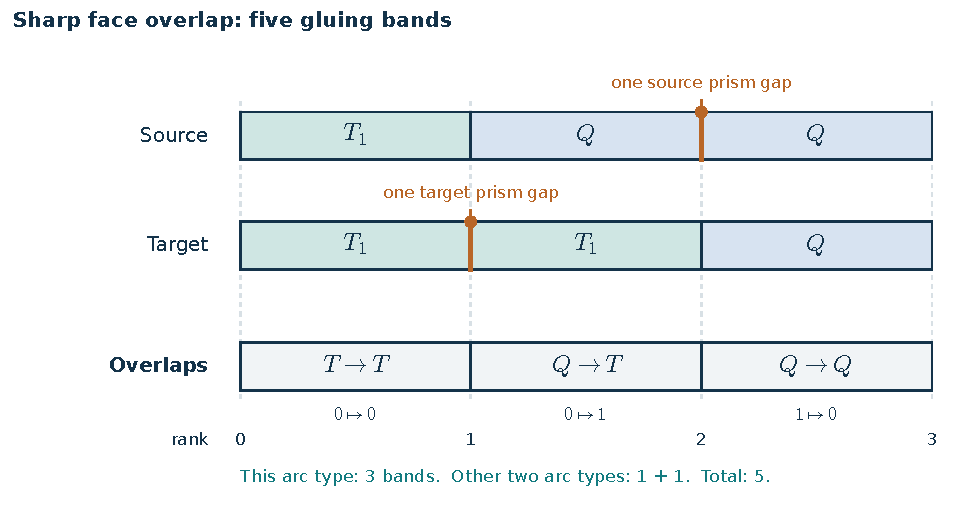
\includegraphics[width=\linewidth]{figures/normal_face_overlap.pdf}
\caption{Sharp local extraction at cut vertex $1$. The source blocks
$[0,1)$ and $[1,3)$ and target blocks $[0,2)$ and $[2,3)$ yield three
pairings. The two other arc types contribute one each, attaining five
bands. Orange marks locate the two singleton prism gaps meeting opposite
residual cells. The lower indices refer to the individual disc stacks.}
\label{fig:normal-face}
\end{figure}

These are local cut data. Around a triangulation edge, one must still
assemble and regularize the incident pieces, reconstruct boundary-pattern
attachments, and identify whole parallelity bundles. The output is not a
claim that the residual-cell labels already form a valid global handle
structure. In particular it is not an implementation of the full
compressed-cut theorem in Lackenby's hierarchy machinery.

\subsection{An explicit interface to interval orbit counting}

Let $n_s$ be the multiplicity of stack $s$, let
$o_s=\sum_{r<s}n_r$, and let $D=\sum_s n_s$.
Concatenate the disc intervals into $[0,D)$. A pairing
$i\mapsto\varepsilon i+c$ from stack $s$ to stack $u$ becomes
\[
 z\longmapsto\varepsilon z+(o_u+c-\varepsilon o_s)
 \quad\hbox{on }[o_s+a,o_s+b).
\]
This conversion is implemented as \texttt{orbit\_input}. Its orbits are
exactly the connected components of the normal surface: a path between
polygon interiors can be moved away from the finite set of polygon
vertices and then crosses a sequence of glued polygon sides. The algorithm
of Agol, Hass, and Thurston~\cite{aht} is the established polynomial-time method for
counting such interval orbits; the new code prepares its input but does
not implement that orbit-reduction algorithm.

The stored cyclic polygon orientations also give a signed version of
each side pairing. If the pairing preserves the two induced boundary
directions, consistent polygon-interior orientations differ by a minus
sign; if it reverses them, the interiors carry the same sign.
The implementation prepares the orientation double cover by making two
copies of every disc and switching copies exactly on negative transports.
If $C$ is the original orbit count and $\widetilde C$ the count in this
double cover, then
\[
 \#\{\text{orientable components}\}=\widetilde C-C,
 \qquad
 \#\{\text{nonorientable components}\}=2C-\widetilde C.
\]
Each orientable component contributes two cover components and each
nonorientable component contributes one. This is an aggregate count;
obtaining the full coordinate vector and topology of each compressed
component requires the weighted orbit machinery or an equally precise
replacement.

\subsection{Validation and measured scope}

The exact geometric oracle realizes triangle slices by
$z_v=1-(j+1)/(4(n+1))$ and quadrilateral slices by
$\sum_{a\in A}z_a=2/3-(j+1)/(3(n+1))$. It explicitly sorts the resulting
face arcs using rational numbers, independently of the block-overlay code.
The suite covers all 24 tetrahedral vertex permutations, four source faces,
and all choices of absent or active quadrilateral type on both sides,
with fixed-seed small multiplicities. It includes 1537 cases, the sharp
example above, and 591 reflected prism bands.

A separate comparison uses Regina~\cite{regina} on 807 small normal-surface inputs.
It compares full component coordinate multisets, Euler characteristics,
orientability, and boundary counts. This includes 92 nonorientable and
274 closed components, scalar multiples of one-sided surfaces, and compatible
normal sums that need not lie on extreme rays. Both interval-orbit adapters
are also checked by explicit finite equivalence relations. Large-coordinate
experiments run only the compressed extractor; neither the reference
expansion nor Regina's component routine is invoked there.

For the previously supplied Fibonacci meridian family at $t=128$, the
input encodes about $2.79\times10^{27}$ normal discs. The extractor returns
764 surface bands, 754 prism bands, 254 prism-to-residue contacts, and
512 local residual cells. At $t=1024$ it returns 6140 surface bands
and 4096 residual cells. Fixed-size tests with two tetrahedra and
65536-bit multiplicities retain ten stacks and four surface bands.
These measurements demonstrate a representation and extraction improvement;
they do not measure a complete unknot-recognition pipeline.

\section{Inherited scalar algebras and conclusive local stopping}
\label{sec:inheritance}

\subsection{The full scalar commutant and its inherited corners}

Work over $k=\mathbb F_2$. Partition the objects of a finite open complex $C$
by their matching, homological degree, and recovered relative quantum shift.
An allowed scalar change of basis is block diagonal for this partition.
Write $b_1,\ldots,b_t$ for the block sizes and
\[
 N=\sum_a b_a,\qquad V=\sum_a b_a^2,\qquad
 A=\operatorname{End}_{\mathrm{sc}}(C)
   \subseteq\bigoplus_a M_{b_a}(k).
\]
The subscript is essential: these are coefficientwise commuting scalar
endomorphisms. They need not be all endomorphisms in the cobordism category.
Every morphism coefficient contributes its own homogeneous linear
commutation equations. The maintained solver computes a complete basis of
$A$ whenever its configured variable cap permits a computation.

\begin{theorem}[Full scalar corner inheritance]
\label{thm:corner}
Let $S$ be an allowed invertible change of basis, and suppose the transformed
complex has an actual direct-sum decomposition
$S^{-1}CS=C_1\oplus\cdots\oplus C_s$, with each $C_i$ a whole connected
component of its differential graph. Scalar blocks on a child carry the
inherited parent labels; fresh relative quantum-shift recovery gives the
same blocks on a connected child. Let $e_i$ be the corresponding
coordinate projection. Then
\[
 \operatorname{End}_{\mathrm{sc}}(C_i)
    \cong e_i(S^{-1}AS)e_i.
\]
In particular, restricting the transported members of any complete vector
space basis of $A$ spans the full scalar endomorphism algebra of $C_i$.
This assertion does not require $e_i$ to be central.
\end{theorem}

\begin{proof}
The coordinate inclusion $j_i$ and projection $p_i$ commute with the
transformed differential, and $p_i j_i=1_{C_i}$. Restriction sends a
parent endomorphism $a$ to $p_iS^{-1}aSj_i$. Conversely, if
$u\in\operatorname{End}_{\mathrm{sc}}(C_i)$, then $j_iup_i$, extended by
zero on all other summands, is a typed scalar endomorphism of the transformed
parent. Thus the restriction map is a surjective linear map, and its image
is precisely the displayed corner algebra. Conjugating back by $S$ proves
the assertion about a basis. All changes preserve the parent quantum
labels. On each connected child the recovered quantum labels differ from
these inherited labels by a constant, so the permitted blocks agree.
\end{proof}

\paragraph{A necessary algebraic distinction.}
The linear map $a\mapsto e_i a e_i$ from the whole parent algebra to its
corner is not in general an algebra homomorphism. For example, in
$M_2(k)$, with $e=E_{11}$, $a=E_{12}$, and $b=E_{21}$, one has
$eabe=e$ while $eae=ebe=0$. Multiplication on the corner itself is
unambiguous; the algorithm needs the surjective linear map, not a quotient
homomorphism assertion about the entire parent algebra.

\begin{lemma}[Canonical-basis compatibility]
\label{lem:canonical-span}
The existing nullspace solver eliminates equations with their most
significant nonzero coordinates as pivots and lists its free variables in
increasing order. Its output is exactly the unique reduced basis of the
solution space whose pivots are least significant nonzero coordinates.
Therefore reducing the restricted spanning vectors to this latter form
produces the same ordered basis as a fresh child commutation solve.
\end{lemma}

\begin{proof}
Each nullspace basis vector has one free coordinate equal to one and all
other free coordinates zero. The equation pivots determined by that free
coordinate occur only at larger indices. Hence the free coordinate is its
least significant nonzero coordinate, and no such pivot coordinate occurs
in another basis vector. These properties characterize reduced row-echelon
form for the reversed choice of pivot direction and determine the basis
uniquely.\end{proof}

This compatibility matters operationally: the bounded basis-prefix search
and the fixed-seed random combinations then inspect exactly the same
candidates, in the same order. General corner inheritance changes the
construction of the search space, not the search policy. With exact
arithmetic and absent an intervening resource interruption, it preserves
the accepted split witnesses and the resulting recursive component order.

\paragraph{Computational scope.}
On a cold recursion tree, general inheritance computes the full scalar
commutant once at the root and derives every subsequently examined child
space by linear algebra, without constructing another commutator system.
An accepted split loaded from an older cache entry need not have a retained
commutant basis; ordinary inheritance can then resume at a descendant.
The cache retains the previous witness format rather than storing large
algebra bases indefinitely.

The implementation has two exact transport kernels. For a low-dimensional
algebra it directly forms $S^{-1}aS$ for its few basis matrices. For a larger
algebra it constructs one packed linear map on matrix variables. The image
of a matrix unit is obtained from
\[
 S^{-1}E_{uv}S=(S^{-1}e_u)(e_v^{\mathsf T}S),
\]
then restricted to all selected children. One application of this packed
linear map transports each parent basis vector. Both kernels give identical
canonical child bases. Their selection affects performance only.

For reference, direct dense transport of a $D$-dimensional algebra costs
$O(D\sum_a b_a^3)$ elementary field operations before child basis
reduction. If child $i$ has $V_i$ scalar variables, reducing $D$ projected
generators costs at most $O(DV_i\min(D,V_i))$ elementary field operations;
packed binary arithmetic improves the corresponding word-operation bound.
These bounds do not imply that transport always beats resolving a sparse
child commutator. The saved quantity is the number of commutator-system
constructions and solves, while the replacement algebra computations have
their own cost. Moreover, cache keys, grading recovery, accepted-witness
verification, and transformation of the differential still inspect
morphism data; the whole recursive scanner is not coefficient independent.

\subsection{A conclusive scalar-locality certificate from dimension saturation}

\begin{theorem}[Dimension-saturated scalar locality]
\label{thm:scalar-locality}
Let $A$ be the complete scalar endomorphism algebra, of dimension $D$, and
let $Q\in A$ have actual minimal polynomial $m_Q(t)$. If
\[
 \deg m_Q=D,
\]
then $A=k[Q]\cong k[t]/(m_Q)$. If in addition
\[
 \dim_k\{p\in k[t]/(m_Q):p^2=p\}=1,
\]
then $C$ has no nontrivial scalar direct-sum decomposition.
\end{theorem}

\begin{proof}
The elements $1,Q,\ldots,Q^{D-1}$ are independent by the definition of the
minimal polynomial. They lie in the $D$-dimensional space $A$ and hence form
a basis. Evaluation therefore identifies the whole algebra $A$ with the
displayed polynomial quotient. In characteristic two, squaring is linear
on this commutative quotient. A one-dimensional fixed space contains exactly
$0$ and $1$, so these are its only idempotents. A nontrivial scalar direct
sum would supply a nonzero nonidentity scalar coordinate idempotent, a
contradiction.\end{proof}

To see the equivalent factorization criterion, write
$m_Q=\prod_{j=1}^r f_j^{e_j}$ with distinct irreducibles $f_j$.
In a primary quotient $k[t]/(f_j^{e_j})$, an idempotent $u$ satisfies
$f_j^{e_j}\mid u(u-1)$. Since $u$ and $u-1$ are coprime, the full
power divides one factor, giving $u=0$ or $1$ in the quotient.
The Chinese remainder theorem therefore gives exactly $2^r$ idempotents,
and the Frobenius fixed space over $\mathbb F_2$ has dimension $r$.
Thus fixed-space dimension one means that $m_Q$ has one distinct
irreducible factor and the quotient is local, including repeated factors.
This argument explains the criterion; the implementation obtains the
fixed space by linear algebra, using the inherited Berlekamp routine
\cite{berlekamp,projectors}, without requiring an integer factorization. A certificate
does not require that the algebra be a field. The tests include both
$\mathbb F_8$ and $\mathbb F_2[t]/((t^2+t+1)^2)$, exhaustively checking that
their displayed commutants have exactly two idempotents.

Both hypotheses are indispensable operationally. The dimension must be that
of the complete commutant, and the polynomial must be the actual minimal
polynomial, not merely an annihilating polynomial. A primary candidate in a
proper subalgebra proves nothing about idempotents elsewhere in $A$.
For example, the identity of a decomposable complex has primary minimal
polynomial $t+1$ while its full commutant has dimension greater than one.
An explicit negative control verifies that this case is rejected.

The implementation reuses the earlier polynomial-projector routine's exact
minimal polynomial and Berlekamp fixed-space computation. When a projector
search fails and its minimal degree equals the full commutant dimension,
the optional locality flag terminates the otherwise bounded candidate
search with a certificate. This shortcut cannot suppress a possible scalar
split: the certificate establishes that none exists. It makes no assertion
about non-scalar cobordism endomorphisms.

The separate verifier recomputes the entire commutant, verifies commutation
of the proposed generator, recomputes its minimal polynomial, and checks
the fixed-space dimension. It deliberately incurs the full cost again;
certificate auditing is outside benchmark timing. Recorded certificates
include all differential rows, matchings, frontier points, and degrees,
and survive JSON round trips.

\subsection{One-generator inheritance on saturated branches}

\begin{corollary}[Inheritance from one saturated generator]
\label{cor:monogenic-corner}
Under the child-label hypotheses of Theorem~\ref{thm:corner},
suppose $A=k[Q]$ has been certified by dimension saturation. For any actual
child coordinate idempotent $e_i$ after an allowed change of basis, its full
endomorphism algebra is generated by the restricted $Q_i$ and its own
identity:
\[
 \operatorname{End}_{\mathrm{sc}}(C_i)=k[Q_i].
\]
Consequently its dimension is $\deg m_{Q_i}$; if $m_{Q_i}$ is primary, the
child is scalar indecomposable without any new commutator solve.
\end{corollary}

\begin{proof}
Conjugation preserves the polynomial-algebra identity. The parent algebra
is commutative, so its child selectors are central. Its corner consists of
the elements $e_ip(Q)e_i=p(Q_i)$, with constants interpreted as multiples
of the corner identity. The corner theorem identifies this with the full
child algebra. Minimal-polynomial dimension and the saturation theorem
now apply.\end{proof}

Thus only one generator needs to be transported, rather than a full parent
basis. The implemented optional path recognizes saturation on an accepted
polynomial-projector witness, transports its original generator, and checks
each examined child's minimal polynomial. A local child is finished
immediately. For a nonlocal child, the powers of the restricted generator
are reduced to the same canonical commutant basis as an independent solve,
and the existing bounded splitter resumes.

There is a stronger algorithmic consequence, which should be distinguished
from the implementation just described. Factoring $m_Q$ into its primary
factors, or recursively using the available polynomial projectors, yields a
complete scalar direct-sum decomposition of a saturated monogenic algebra
when split budgets permit. The current implementation completely finishes
the measured two-field branches; it does not replace every nonlocal child's
bounded search by an unlimited recursive factor-decomposition procedure.

\subsection{Controlled families and precise performance claims}

For the existing attached-copy family with $r\geq2$ copies, the commutant is
$M_r(k)$, there are $3r^2$ scalar variables, and each size-$r$ solve builds
$2r^2$ nonzero coefficient equations. With sufficiently large split budget,
the original deterministic policy splits off one copy at each step. Its
total equation construction count is therefore
\[
 2\sum_{j=2}^r j^2
   =\frac{r(r+1)(2r+1)}3-2,
\]
whereas inheritance builds exactly $2r^2$ such equations at the root. This
is an exact cubic-to-quadratic reduction in the number of constructed
commutator equations, not a claim of a corresponding total runtime bound.
The basis candidates and accepted witnesses remain identical. Both the
formula and the witness identity are regression tested through $r=16$.

The separately inherited two-field fixtures have a homogeneous two-term
differential $d=xI+yB$ over a two-dot algebra, where $B$ is conjugate to
companion matrices for two distinct irreducibles of degree $r$. Comparing
the independent $x$ and $y$ coefficients shows that a scalar endomorphism
is a common matrix commuting with $B$. Thus
\[
 \operatorname{End}_{\mathrm{sc}}(C)
  \cong k[t]/(fg)\cong\mathbb F_{2^r}\times\mathbb F_{2^r}.
\]
These are legitimate graded algebraic complexes, without a claimed
realization as knot-scan prefixes. Their root has $8r^2$ scalar variables.
For the recorded dense fixtures at $r=8,10,12$, the accepted generator
saturates the algebra. One root commutant solve, two candidate tests, and
two inherited scalar-locality certificates complete the decomposition.
The earlier primary policy used respectively $46,52,58$ candidates over
the whole recursive compression and three commutant computations.

Natural-knot scans, attached-copy tests, and field-algebra tests have separate
timing scopes. The benchmark retains randomized paired samples and A/A
controls. It compares general inheritance alone, local stopping alone,
their ordinary combination, and one-generator inheritance independently.
No controlled-family speedup establishes a worst-case bound for arbitrary
knot diagrams. In particular, nothing here bounds the number of objects,
matching types, algebra variables, or scalar-indecomposable summands of a
general scan by a quasipolynomial function of its crossing number.

\paragraph{Provenance and proposed follow-up questions.}
The polynomial-projector module and the two-field fixtures are reproduced
unchanged from the earlier October 8 projectors package~\cite{projectors}, with their hashes
recorded separately. Their algorithm is prior work, not a new contribution
of this continuation. The additions are complete-corner transport,
canonical basis preservation, dimension-saturation stopping and verification,
and one-generator inheritance on certified saturated branches.

The next questions are whether to replace the residual bounded scalar search
by constructive finite-algebra radical and semisimple-quotient algorithms;
whether an exact cost model can select transport versus resolving a sparse
commutator; whether additional natural knot families produce saturated or
otherwise tractable scalar algebras; and which structural bounds control
the number and size of scalar-indecomposable components. Extending reuse
across the addition of a crossing is a different problem: a child corner
of the same complex inherits all endomorphisms by extension by zero, while
a newly glued complex can gain endomorphisms that have no ancestor.

\section{Global complexity: a precise remaining target}
\label{sec:global}

\subsection{The family-query bound removes one parameter explosion}

Suppose a represented stage previously tried up to $m^k$ phase vectors,
and the only information requested from that family is feasibility and
the minimum number of cyclic covering components. For the affine model
of this article, compilation and optimization have polynomial bit cost
in the listed matrix dimensions and input integer lengths. Thus the
$m^k$ term can genuinely be removed from that stage. The emitted witness
and its independent verification are polynomial as well. This conclusion
does not require $k=O(\log n)$ or $m$ to be a small integer.

There is no corresponding conclusion for a stage which must distinguish
all seam assignments under future attachments, require many selected
boundary preimages to be connected, or test unknown normal-surface
embeddings. Sections~\ref{sec:surface-families} and \ref{sec:boundaries}
give examples and formal barriers to those extensions.

\subsection{A composition theorem with every hypothesis exposed}

\begin{theorem}[Conditional represented-algorithm bound]
\label{thm:conditional-global}
Consider a complete unknot-recognition algorithm on $n$-crossing diagrams.
Suppose that, on every execution:
\begin{enumerate}
\item the number of represented states and transitions, including all
failed branches and resets, is at most $\exp(C\log^2(n+2))$;
\item every listed state and certificate has bit size at most
$\exp(C\log^2(n+2))$;
\item every transition is either a verified operation proved polynomial
in that bit size, or another routine whose total cost has the same
quasi-polynomial bound;
\item the representation and transition relation are sound and complete
for the required topological decision.
\end{enumerate}
Then the total bit time, including certificate checks and output, is
$\exp(O(\log^2(n+2)))$.
\end{theorem}
\begin{proof}
A fixed polynomial in $\exp(C\log^2(n+2))$ is
$\exp(O(\log^2(n+2)))$. Multiplying this by the assumed bound on the
number of transitions preserves the form. Reading and emitting every
state is included in the same product. The soundness and completeness
hypothesis is needed to identify the resulting algorithm as a complete
recognizer rather than an exact subroutine or a partial search.
\end{proof}

This bookkeeping theorem is elementary. Its usefulness is diagnostic:
the arithmetic optimizer and normal-coordinate extractor establish
particular transition-cost statements in item (3), under their explicit
input contracts. Scalar-space inheritance avoids repeated work on an
already represented complex. None establishes items (1), (2), or (4) for
unrestricted knots. In particular, the theorem is not presented as a
new solution to the central complexity problem.

\subsection{Why a termination potential is insufficient}

A lexicographically decreasing list with $L$ entries each in
$\{0,\ldots,g\}$ can visit $(g+1)^L$ values. The corresponding integer
potential is
\[
 P(a_1,\ldots,a_L)=\sum_{i=1}^L a_i(g+1)^{L-i}.
\]
Decreasing an earlier coordinate and resetting all later coordinates to
$g$ decreases $P$, but can make progress of only one unit. This is exactly
the type of accounting behind the hierarchy iteration bound
$L(g+1)^L$ in Lackenby's Proposition 9.1~\cite{lackenby2026}.

A sufficient numerical regime for this particular bound is
\[
 \log(L+1)+L\log(g+1)=O(\log^2(n+2)),
\]
together with control of the per-step bit cost. The first term also
covers $g=0$, when the bound reduces to $L$. A merely linear estimate
for $L$ does not supply it. Faster gcds, shorter certificates, or reduced
commutant solves do not change the number of possible resets. A new
global argument would need, for example, a stronger amortized progress
measure, a decomposition theorem limiting genuinely new states, or
an operation that processes a whole relevant reset family symbolically.

\subsection{The two geometric interfaces must not be conflated}

The normal extractor produces partial signed interval maps, with source
and target stacks and explicit endpoint data. The family optimizer
receives total translations of a common cyclic fibre and affine
parameter constraints. These are different mathematical objects. A
sound bridge could identify a cyclic block inside the interval data,
certify that all its possible completions are represented, and pass the
induced congruences to the optimizer. No such general bridge is included.

Likewise, computing the local complement cells is less than constructing
their full residual handle structure, including every attachment and
boundary pattern. General orbit counting can determine connected pieces,
but subsequent genus, orientation, and vertical-annulus data must retain
the appropriate provenance. Theorem 14.4 of the geometric literature
identifies the desired full uniform-type handle-structure interface~\cite{lackenby2026}; the present
implementation supplies a concrete first portion of it.

\subsection{The algebraic route retains its intrinsic size barrier}

Transporting an endomorphism space can avoid repeatedly solving for the
same information. A certified local scalar endomorphism algebra can stop
a futile search for scalar direct summands. Neither fact bounds the
number of surviving homological generators or the size of the parent
commutant. A complex with a local endomorphism algebra can still be large.
The first computation of that algebra may dominate, and a bounded search
can remain inconclusive when no dimension-saturated generator is found.

The measured implementation therefore retains caps, transactional failure
behavior, and separate optional controls. A local algebra certificate
means ``no nontrivial splitting by the admitted scalar maps.'' It does
not mean ``unknot,'' ``small homology,'' or ``no more general
continuation-compatible compression.''

\section{Implementation, independent checks, and measured performance}
\label{sec:experiments}

\subsection{Evidence and timing conventions}

The proofs establish asymptotic claims for their stated input models.
Independent finite checks test whether the implementation realizes those
models. Timings answer a narrower question about the cost of these particular
implementations in the recorded environment. These three forms of evidence
are reported separately.

The recorded runtime was Python 3.12.14 on Linux x86\_64, kernel 6.18.44,
with glibc 2.39. The optional native geometry audit used the Regina 7.4.1
Python distribution; its library version string reports 7.4. Computations
ran in a shared environment without CPU isolation. Absolute elapsed times
should therefore be treated as descriptive measurements, not portable
performance predictions. In particular, repeated geometry runs varied under
shared load. The final recorded JSON files, rather than earlier working
measurements, supply every table below.

The arithmetic measurements use three repetitions per input and include
certificate generation and the optimizer's independent certificate check.
Normal extraction uses five repetitions on the layered-torus sequence and
seven for fixed triangulation size. Fixtures are built before these timed
regions. No expanded surface or native component computation is called on
the large normal-coordinate cases.

The scalar benchmark uses seven randomized paired rounds. Each arm has a
fresh state, an untimed warm-up, and between one and five calls per round,
with batch size recorded in the data. A/A controls run the reference twice.
A reported ratio is
\[
 \operatorname{median}_{j=1}^7\frac{T_{\mathrm{reference},j}}
                                      {T_{\mathrm{variant},j}},
\]
so values greater than one favor the variant. This differs in general from
the ratio of the two separately reported median times. Exact output
comparisons and scalar-locality certificate audits are outside these timed
regions. No confidence interval or natural-knot speedup is inferred from a
few percent of timing variation.

\subsection{Arithmetic correctness and binary-size stress cases}

The standalone arithmetic tests use exhaustive enumeration of the original
variables as the reference, not the parameterization returned by the new
solver. The exhaustive and seeded comparisons total:

\begin{center}
\small
\begin{tabular}{lr}
\toprule
Independent arithmetic comparison & Cases\\
\midrule
Scalar merges, $m\le48$ & 38\,024\\
Two-coordinate merges, $m\le8$ & 8\,772\\
Two-generator scalar cosets, $m\le10$ & 3\,025\\
Scalar congruences, $m\le24$ & 4\,900\\
$2\times2$ systems, $m\le4$ & 4\,890\\
One-variable one-seam families, $m\le6$ & 2\,275\\
Seeded dense random families & 2\,000\\
\textbf{Total} & \textbf{63\,886}\\
\bottomrule
\end{tabular}
\end{center}


Additional tests cover empty parameter and holonomy dimensions, modulus one,
cooperative cancellation, malformed input, and deliberately corrupted
certificates. The corresponding thirteen \code{unittest} methods are
included in the integrated suite. The verifier can be run without calling
the optimizer or trusting a supplied kernel basis.

\begin{center}
\small
\begin{tabular}{lrrrr}
\toprule
Family & Modulus bits & $n/q/\beta$ & Min. & Seconds\\
\midrule
$2+z$, no seams & 2\,648 & 1/0/1 & 1 & 0.000081\\
$2+z$, no seams & 42\,353 & 1/0/1 & 1 & 0.008106\\
$2+z$, no seams & 169\,409 & 1/0/1 & 1 & 0.191455\\
Dense constrained & 131 & 24/12/7 & 6 & 0.019229\\
Dense constrained & 515 & 24/12/7 & 6 & 0.039649\\
Dense constrained & 2\,051 & 24/12/7 & 6 & 0.231718\\
Dense constrained & 8\,195 & 24/12/7 & 6 & 2.446944\\
\bottomrule
\end{tabular}
\end{center}


Here $n/q/\beta$ gives the variable, constraint, and holonomy dimensions.
For the last one-parameter row, $m=6^{65536}$ has 169,409 bits. The returned
witness is $z=3^{65536}$, and exactly seventeen saturation gcds are used.
The algorithm represents no individual sheets and enumerates no parameter
tuples. Its work is controlled by binary length, not by the astronomical
integer value of $m$.

The dense stress families have a deliberately planted exact optimum six.
For a seeded dense matrix $A$, a feasible hidden vector has every coordinate
divisible by six. The first six holonomy rows are $A_j+6R_j$, and the last
holonomy is the constant six. On the feasible locus all coordinates are
multiples of six, and the last coordinate forces their gcd with $m$ to be
six. The returned certificates have six nonzero dual entries. This design
provides a known independent answer while exercising dense congruence
elimination and nontrivial dual certificates; it is not presented as a
sample of difficult knot exteriors.

\subsection{Surface-family compilation and query boundaries}

The geometric wrapper has nineteen regression methods. Its seeded test
constructs 120 families, of which 51 are feasible and 69 are infeasible.
It examines 1,337 original parameter assignments: 437 satisfy the seams,
and 900 fail them. For each feasible assignment, a direct disjoint-set
calculation on patch--sheet pairs agrees with the compiled component count.
This reference does not use spanning-tree potentials or the compiled loop
list. Every family's minimum and feasible-assignment count agree with the
literal results, and both kinds of certificate verify.

Targeted cases check a tree edge traversed backwards, reversal of a seam,
nonorientable peripheral squares, both base-boundary degrees, and gluing
that connects locally disconnected covers. The emitted large-integer JSON
certificates also survive a serialize--parse--verify round trip. This last
check is material: a verifier that accepts a large integer in memory but
rejects its documented hexadecimal transport is not a usable artifact
verifier. The wrapper decodes only documented certificate integer fields;
it does not interpret unrelated metadata as mathematics.

A separate check of Theorem~\ref{thm:peripheral-hardness} uses the maintained
surface-cover classifier to inspect the full lifted-boundary profiles for
all 351 assignments of three graph families:

\begin{center}
\small
\begin{tabular}{lrrr}
\toprule
Graph & Assignments & Globally connected & \shortstack{All designated\\boundaries connected}\\
\midrule
$K_3$ & 27 & 24 & 6\\
$K_4$ & 81 & 78 & 0\\
$C_5$ & 243 & 240 & 30\\
\bottomrule
\end{tabular}
\end{center}

These checks are distinct from the 63,886 arithmetic cases. The $K_4$
example makes the interface boundary concrete: a family can have many
globally connected members and no member satisfying all requested
peripheral connectedness conditions.

\subsection{Normal-coordinate extraction: exact geometric and native audits}

The local geometric oracle realizes triangle and quadrilateral discs by
rational barycentric levels and sorts the actual face intersections.
Its 1,537 cases cover all 24 vertex permutations, all four source faces,
and all absent/active quadrilateral combinations on each side. The two
methods agree on 9,771 individual disc identifications and 4,850 prism-gap
identifications. The latter include 591 reflected bands, which exercise
the otherwise easy-to-miss $-1$ in the reflected gap map.

A separate Regina comparison covers 807 small normal-surface inputs and
1,537 component coordinate/topology records, including 92 nonorientable
and 274 closed components. It checks full component-coordinate multisets,
Euler characteristics, orientability, and boundary counts. Scalar multiples
of one-sided surfaces and compatible nonextreme sums are included.
Eight additional package tests exercise the command-line interface,
callbacks, schema errors, matching failures, empty surfaces, and binary
coordinate transport. These finite comparisons support the implementation;
they do not replace the extraction proof.

For the Fibonacci meridian family inherited from the earlier certificate
report, the final measurements are:

\begin{center}
\small
\begin{tabular}{rrrrrrr}
\toprule
$t$ & Coordinate bits & Surface & Prism & Contacts & Residue & ms\\
\midrule
8 & 108 & 44 & 34 & 14 & 32 & 0.833\\
16 & 342 & 92 & 82 & 30 & 64 & 1.679\\
32 & 1\,214 & 188 & 178 & 62 & 128 & 3.533\\
64 & 4\,554 & 380 & 370 & 126 & 256 & 7.162\\
128 & 17\,635 & 764 & 754 & 254 & 512 & 15.081\\
256 & 69\,391 & 1532 & 1522 & 510 & 1024 & 20.934\\
512 & 275\,267 & 3068 & 3058 & 1022 & 2048 & 57.337\\
1024 & 1\,096\,505 & 6140 & 6130 & 2046 & 4096 & 115.382\\
\bottomrule
\end{tabular}
\end{center}


``Coordinate bits'' is the sum of the binary coordinate lengths, with one
bit charged for zero; it is not the maximum coordinate length. ``Surface''
and ``Prism'' count face-pairing bands, ``Contacts'' counts the exceptional
prism-to-residue contacts, and ``Residue'' counts local residual cells.
At $t=128$ the input represents exactly
\[
 2\,791\,715\,456\,571\,051\,233\,611\,642\,548
\]
normal discs, but only 764 surface bands and 754 prism bands are produced.
For two fixed tetrahedra with 65,536-bit multiplicities, there remain ten
stacks, four surface bands, and four prism bands; the recorded seven-run
median is 0.000600 seconds. These are representation and extraction
measurements. They do not include general orbit reduction, parallelity
bundle recognition, or a complete hierarchy iteration.

\begin{figure}[tb]
\centering
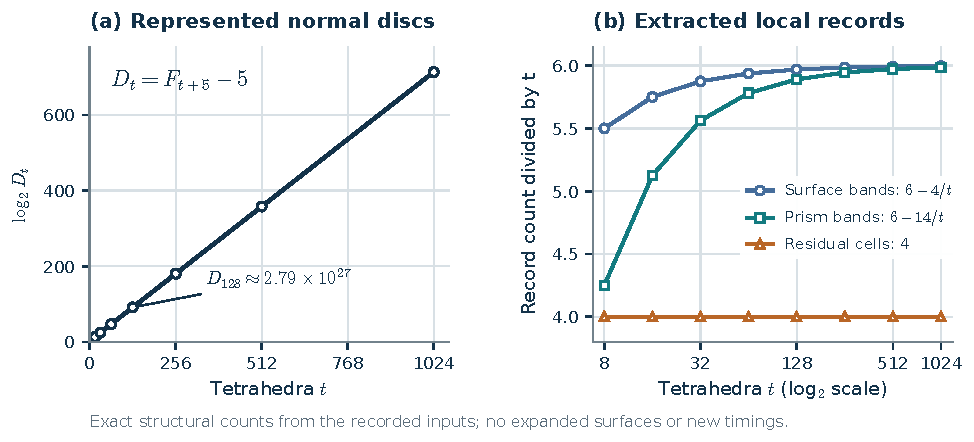
\includegraphics[width=\linewidth]{figures/normal_extraction_scaling.pdf}
\caption{Exact structural counts for the inherited Fibonacci meridian
family, at the recorded values $t=8,\ldots,1024$. The normal-disc count
is $D_t=F_{t+5}-5$. Its binary logarithm grows linearly with $t$ in
panel (a), while panel (b) shows bounded numbers of extracted records per
tetrahedron. The horizontal axes use different scales, as labelled.
These are count data, with no fitted running-time exponent.}
\label{fig:normal-scaling}
\end{figure}

\subsection{Attached copies: exact equation savings and a crossover}

The attached-copy benchmark compares the modified backend with the pinned
\code{scalar_split.py}; both use the same remaining dependency modules.
The measured region is recursive scalar compression followed by component
sharing. Fixture construction is outside the timed region.

\begin{center}
\small
\begin{tabular}{rrrrrrr}
\toprule
$r$ & Old equations & Inherited & Old solves & New & Ratio & A/A\\
\midrule
4 & 58 & 32 & 3 & 1 & 0.848 & 1.027\\
8 & 406 & 128 & 7 & 1 & 1.099 & 1.051\\
12 & 1\,298 & 288 & 11 & 1 & 1.252 & 1.013\\
16 & 2\,990 & 512 & 15 & 1 & 1.468 & 0.999\\
24 & 9\,798 & 1\,152 & 23 & 1 & 1.759 & 0.989\\
\bottomrule
\end{tabular}
\end{center}


The equation counts are the exact values proved in
Section~\ref{sec:inheritance}. At $r=16$, repeated solves construct 2,990
nonzero equations across fifteen commutant computations, while inheritance
constructs 512 equations in one computation. Candidate order and accepted
split witnesses agree. The 1.468 paired ratio reflects an actual measured
benefit. At $r=4$, the ratio 0.848 instead shows the cost of transport and
canonicalization exceeding the saving.

The $r=24$ experiment raises the backend caps: its 72 objects and 1,728
scalar variables exceed the default limits, and its 23 splits exceed the
default split budget of sixteen. It is a controlled scaling experiment,
not a claim about behavior under default caps. The $r\le16$ rows fit the
default object and variable limits. Neither the exact cubic-to-quadratic
equation reduction nor the measured ratios establish an analogous total
bit-time exponent for arbitrary complexes.

\subsection{Field algebras: identify the work that actually matters}

For the dense two-field family, the reference is the previously supplied
primary-projector policy, with descendant commutants recomputed. This is
a separate reference from the pinned zero-primary Fitting search used for
the preceding table. The new mechanisms are measured independently:

\begin{center}
\small
\begin{tabular}{rrrrrr}
\toprule
$r$ & Inheritance & Local stop & Both & One generator & A/A\\
\midrule
8 & 0.890 & 1.877 & 1.446 & 2.165 & 1.003\\
10 & 0.868 & 2.033 & 1.565 & 2.312 & 1.002\\
12 & 0.895 & 1.935 & 1.489 & 2.229 & 0.985\\
\bottomrule
\end{tabular}
\end{center}


The four variant columns mean general corner inheritance only, direct
saturation-locality stopping only, their ordinary combination, and the
one-generator corner path with locality certification. General inheritance
alone is slower in all three displayed cases. Carrying the full basis is
not the right optimization for these low-dimensional commutative algebras.
The saturated generator exposes the complete algebra and finishes both
local children directly.

For degrees $r=8,10,12$, the old candidate counts are respectively
46, 52, and 58. The one-generator path uses two candidate tests and one
commutant computation, followed by two scalar-locality certificates.
The reference uses three commutant computations. The corresponding paired
ratios are 2.165, 2.312, and 2.229. The $r=12$ root has 1,152 scalar
variables, exceeding the default variable cap, although its 48 objects
fit the default object cap.

The data also retain lower-degree cases and a degree-eight case using only
one elementary change of basis to mix the two blocks. Not every accepted generator saturates the algebra; the latter case
falls back to ordinary inheritance, and direct local stopping is faster.
This is evidence for a cost-aware choice of mechanism, rather than for
turning every optional feature on unconditionally. All these fixtures are
legitimate homogeneous algebraic complexes; no realization as natural knot
scan prefixes is claimed.

\subsection{Natural scans: a useful negative timing result}

Natural examples measure a complete raw Khovanov scan, including scanner
construction, at the same preselected order for every arm. Loading the
input and finding that order are excluded. Homological ranks and the
configured capped decisions are checked independently. The timing table is:

\begin{center}
\small
\begin{tabular}{lrrrrrl}
\toprule
Diagram & Crossings & Old ms & Inherit & One gen. & A/A & Solves\\
\midrule
Trefoil & 3 & 0.319 & 0.961 & 0.958 & 1.003 & 0\,$\to$\,0\\
Conway & 11 & 7.530 & 0.990 & 1.018 & 0.954 & 10\,$\to$\,7\\
Kinoshita--Terasaka & 11 & 8.079 & 1.022 & 1.010 & 1.016 & 9\,$\to$\,6\\
Hard unknot 8 & 8 & 0.732 & 1.001 & 0.993 & 1.002 & 0\,$\to$\,0\\
Stress braid 5/36 & 36 & 457.241 & 1.021 & 0.980 & 1.005 & 5\,$\to$\,5\\
$T(3,5)$ & 10 & 2.917 & 0.998 & 0.994 & 0.982 & 0\,$\to$\,0\\
\bottomrule
\end{tabular}
\end{center}


The final column counts actual commutant computations; for the historical
arm, cache misses equal those computations in these cases. Conway falls
from ten to seven and Kinoshita--Terasaka from nine to six, each using three
inherited child spaces across two Fitting splits. There is a real reduction
in repeated algebra construction. Wall-time inheritance ratios, however,
range only from 0.961 to 1.022, comparable with the control variability.
These measurements support no convincing natural-knot wall-time speedup.
No natural example in this sample activates a primary split, a conclusive
locality certificate, or a monogenic corner. The controlled field gains
must remain separate from claims about the complete recognizer.

\subsection{Integrated regression and the inherited worker correction}

The untouched pinned baseline ran 725 tests: 724 passed and one failed.
The failure in \code{test_communication_retains_input_across_polls} was
reproduced in isolation. Repeating \code{communicate} with the input
removed after a timeout could leave a large worker request only partially
written in the current Python runtime. The earlier projectors archive
already contained a single-submission communication-thread correction.
We copied that correction exactly and attribute it as inherited work.
It is not counted as a new performance theorem or optimization.

The complete staged source bundle then passed \textbf{790 tests}, with no
failures, in 110.342 seconds of reported test-runner time. This includes all
725 baseline methods, twelve restored tests for the inherited primary
projector module, and 53 new arithmetic, family, normal-extraction, and
inheritance/locality methods. Targeted scalar checks also preserve cache,
cap, cancellation, grading, and transactional behavior. The logs are
included, including the original baseline failure; the differing total
suite times are not used as a performance comparison.

\section{Further research questions and prioritized experiments}
\label{sec:research}

The most useful next work should connect the proved interfaces to
genuine residual knot instances. The following questions are proposed
targets, not claims that each formulation is absent from the literature.

\subsection{From normal coordinates to a complete compressed cut}

\begin{enumerate}
\item \textbf{Complete the residual face attachment map.} The current
extractor identifies local non-prism cells and their prism contacts.
Construct all residual faces, edges, and their identifications, with an
independent expanded oracle on small normal surfaces. The acceptance
criterion is a complete cut manifold representation, not only correct
piece counts.
\item \textbf{Connect a general interval-orbit implementation.} Concatenate
the signed bands into the integer-interval format of
Agol--Hass--Thurston and compute connected components without expansion.
Then add weighted orbit data for Euler characteristic, boundary count,
and orientability. An existing independent orbit implementation can be
used as a comparison oracle, with its provenance retained.
\item \textbf{Certify cyclic blocks inside interval data.} Find conditions
under which a family of partial interval maps is equivalent to total
translations on a common cyclic fibre. Return the equivalence and
attachment transport as a checkable witness. This is the missing bridge
between the two geometric kernels in this article.
\item \textbf{Follow actual nonextreme normal surfaces.} The earlier
primitive-extreme-ray disc checker deliberately avoids component
enumeration. Test the new extractor on connected and disconnected
nonextreme sums, one-sided surfaces, boundary-parallel surfaces, and
normal surfaces with large quadrilateral coordinates. Those examples
exercise cases not certified by primitivity alone.
\item \textbf{Track boundary patterns through compression.} Extend local
provenance to pattern arcs and vertical annuli. A useful milestone is one
complete verified iteration of the geometric hierarchy on a knot
exterior, including the boundary-pattern update and a replayable
certificate.
\end{enumerate}

\subsection{Stronger symbolic queries with controlled expressiveness}

\begin{enumerate}[resume]
\item \textbf{Geometrically restricted peripheral constraints.} The
three-colouring reduction shows that arbitrary simultaneous peripheral
connectedness is too expressive for an unrestricted polynomial claim.
Identify geometric restrictions, such as bounded incidence width or a
fixed number of designated boundaries, that yield tractable subclasses.
\item \textbf{Fixed-sign dihedral families.} If reflection signs are fixed
and only shifts vary affinely, determine which component-minimization
questions reduce to a bounded number of affine-gcd problems. Treat
parity, fixed residues, and the small moduli $1,2$ explicitly.
\item \textbf{Joint objectives for disconnected bases.} The two-component
counterexample shows that independent minima cannot simply be added.
Study fixed-parameter algorithms in the number of base components or in
the incidence graph between parameter variables and component objectives.
\item \textbf{Boundary-profile existence.} Seek algorithms for one or a
fixed number of prescribed boundary-cycle profiles. Distinguish a
bounded disjunction of congruence systems from a claim that all possible
genus and boundary constraints are polynomial.
\item \textbf{Counting with supplied arithmetic structure.} Given a
factorization of $m$, implement the exact prime-local count formula and
compare it with enumeration on small cases. Without a factorization,
study partial counts or certificates that do not implicitly solve the
totient problem.
\end{enumerate}

\subsection{Scalar compression and actual scanner activation}

\begin{enumerate}[resume]
\item \textbf{Measure natural commutant reuse.} Record parent algebra
dimension, actual child dimensions, equation counts, transport costs,
and candidate counts on difficult prime knots that survive early
filters. A controlled algebraic speedup should not be reported as a
complete-recognizer improvement without this measurement.
\item \textbf{Discover saturated generators efficiently.} A generator
$Q$ with $\dim\F_2[Q]=\dim\End(C)$ supplies a complete commutative
description. Study deterministic candidate construction and characterize
which scalar algebras admit such a generator. Noncommutative or
nonmonogenic algebras require a different certificate.
\item \textbf{Certificates for larger nonsplit algebras.} Generalize the
locality certificate to noncommutative finite-dimensional scalar
algebras using their radical and semisimple quotient. Charge both the
cost of obtaining the algebra and the cost of the certificate.
\item \textbf{Continuation-compatible inheritance.} Determine which
parts of an endomorphism-space description survive the next crossing
attachment. Arbitrary reuse across changed differentials is unsound;
the update must prove the relevant intertwining conditions.
\item \textbf{Formalize the small arithmetic core.} The affine merge lemma,
bounded-residue congruence elimination, and dual verifier are suitable
for a compact Lean formalization. The proof should include the
composite-modulus case and the exact meaning of the bit-cost model.
\end{enumerate}

\subsection{A credible route to the global target}

\begin{enumerate}[resume]
\item \textbf{Prove an amortized hierarchy reset bound.} A natural target
is a quantity whose total loss bounds all failed repairs and is only
quasi-polynomial in the original diagram size. Merely restating a
lexicographic termination proof is not enough.
\item \textbf{Bound the encoding of every reachable state.} Include
normal weights, boundary patterns, attachment maps, coefficient sizes,
and any family parameters. A finite number of local topological types
does not by itself bound the multiplicity or marking data.
\item \textbf{Find a complete residual family with proven coverage.}
Choose an explicit infinite class that defeats inexpensive existing
certificates, and prove that the remaining geometry always enters the
implemented compressed model. This would be more informative than a
large synthetic speedup alone, even if the resulting theorem remains
restricted to that class.
\end{enumerate}

\section{Reproducibility and repository integration}
\label{sec:reproduce}

\subsection{What the archive contains}

The archive includes the complete article source, generated tables and
scientific figures, and the compiled PDF. A curated \code{source/} tree
contains the maintained Python implementation, its tests and fixtures, and
the historical reference modules required by those tests. Historical result
archives unrelated to this continuation are omitted. The distributed source
is pinned to \sourcepin{} except for the explicit delta in
\code{source_manifest.json}.

The \code{patches/} directory contains a Git-applicable patch with two
modified files and fourteen new files. A separate \code{baseline/} directory
retains the two modified files exactly as they appeared at the pinned
revision. It lets the scalar benchmark load its historical arm without
network access or a Git checkout. Independent validation applied the patch
in a fresh directory, checked all sixteen affected outputs byte for byte,
and compared every one of the 362 distributed source files with the working
tree. The 346 unmodified source files match the pinned Git blobs exactly.

The \code{experiments/} directory contains the arithmetic and geometric
reference checks, including rational geometry and optional Regina
comparisons. \code{results/} preserves the recorded measurements and exact
comparison counts. \code{validation/} preserves the baseline failure,
final 790-test success, targeted checks, patch audit, and artifact checks.
Standalone copies of the small arithmetic and extraction modules are kept
only to make those experiment scripts independent of package installation;
their bytes match the corresponding integrated modules.

\subsection{Commands for independent reproduction}

The new mathematical kernels require only the Python standard library.
Regina is optional for the independent native audit; Matplotlib is optional
for regenerating the figures. The recorded versions are listed in
\code{requirements-audit.txt}. LaTeX compilation uses ordinary
\code{pdflatex} and \code{latexmk}, with the packages declared in the main
source file.

\noindent\begin{minipage}{\linewidth}
From the extracted archive root:

\begin{lstlisting}
python scripts/check_hashes.py
python scripts/reproduce.py quick

# Optional native audit and figure dependencies:
python -m pip install -r requirements-audit.txt
python scripts/reproduce.py full

# Paired and binary-size benchmarks:
python scripts/reproduce.py benchmarks

# Rebuild the article:
cd article
latexmk -pdf -interaction=nonstopmode -halt-on-error \
  unknot_affine_families.tex
\end{lstlisting}
\end{minipage}

The reproduction driver writes new logs and measurements to
\code{reproduction/}; it preserves the recorded evidence. ``Quick'' runs
all 65 methods in the five new or restored test modules, the rational
face-order audit, the certificate examples, and the peripheral reduction
check. ``Full'' runs the complete integrated suite and the Regina audit.
The benchmark mode is separate so that correctness checks do not depend
on machine-specific timing thresholds.

To review the source delta at the pinned repository revision, use:

\begin{lstlisting}
git apply --check /path/to/affine_families_and_inheritance.patch
git apply /path/to/affine_families_and_inheritance.patch
\end{lstlisting}

The article and supporting research files can then be placed in the
repository's chosen report or incoming-document location. The distributed
patch edits the implementation paths; it does not choose or overwrite a
report number.

\subsection{Concrete example contracts}

The cyclic-family examples include a constrained annulus with optimum two,
a self-seam joining twelve locally disconnected annuli into a connected
member, an infeasible seam with a negative certificate, and a 10,589-bit
modulus whose stored hexadecimal witness verifies without sheet expansion.
The $K_4$ example keeps its designated-boundary requirements in a separate
metadata file, since that hard peripheral query is outside the optimizer's
strict input schema. Run:

\begin{lstlisting}
python scripts/check_family_examples.py
\end{lstlisting}

For direct package use, the public family functions are
\code{compile_family}, \code{optimize_cover_family},
\code{realize_family}, and \code{verify_cover_family_certificate} in
\code{fastunknot.cyclic_cover_family}. The command-line entry point accepts
one JSON input and emits the compiled family and arithmetic certificate.
The verifier ignores the producer's compilation and recomputes it from the
original geometry. It certifies feasibility and optimality, or infeasibility;
it does not certify the auxiliary assignment count or any topological
predicate outside the stated component objective.

The normal extractor accepts a JSON object with exactly
\code{triangulation} and \code{coordinates}. It emits the signed polygon
bands, prism bands, residual-cell incidence data, and provenance.
The optional \code{--orbit-input surface} and
\code{--orbit-input orientation} switches emit the corresponding interval
orbit problems. Those files are inputs to a subsequent orbit engine, not
claims that the engine has been run. The supplied normal examples include
the sharp two-tetrahedron fixture and a 128-tetrahedron Fibonacci meridian.

\subsection{Optional scalar controls and evidence boundaries}

Within the already optional Fitting backend, ordinary reuse defaults to
\code{fitting_reuse_endomorphisms=True}. It preserves the deterministic
candidate basis and search policy. The separately configurable primary,
locality, and one-generator paths default to false:

\begin{lstlisting}
from fastunknot.scalar_split import fitting_khovanov_rank
answer = fitting_khovanov_rank(
    pd,
    fitting_reuse_endomorphisms=True,
    fitting_primary=True,
    fitting_certify_local=True,
    fitting_monogenic_corners=True,
)
\end{lstlisting}

This snippet deliberately selects an experimental backend and its optional
mechanisms. It is not a recommendation to raise every size cap on arbitrary
inputs. Independent locality auditing uses
\code{verify_scalar_local_certificate}; unlike production inheritance,
that verifier recomputes the full commutant to check the dimension claim.
The different cost contracts of the arithmetic and scalar verifiers should
not be conflated.

\subsection{Provenance and continuing obligations}

The inherited polynomial-projector module, its fixtures and tests, and the
worker-communication correction are attributed by source path and hash.
The Fibonacci meridian family is likewise attributed to the earlier
compressed-certificate report. No external article PDF or downloaded slide
deck is bundled as a new research artifact. The new work follows the
repository's MIT No Attribution license; included pre-existing components
retain their accompanying license notices.

A claim ledger records proved statements, tested implementation contracts,
measured improvements, negative results, and unresolved global obligations.
The immediate deliverable is a set of exact reusable operations and an
integration-ready research record. A complete quasi-polynomial recognizer
still requires the explicit state-growth, representation-size, and
geometric-coverage arguments in Section~\ref{sec:global}.

\begin{thebibliography}{99}
\raggedright
\bibitem{repo}
V.~Reshetnikov, \emph{ProveIt, Topology/UnknotRecognition}.
Repository revision \sourcepin, inspected 8 October 2026.
\url{https://github.com/VladimirReshetnikov/ProveIt/tree/ea9cf443c8ce33e09ed0c48b0ef7856ddf6326a3/Topology/UnknotRecognition}.

\bibitem{projectors}
ProveIt research continuation, \emph{Polynomial Projectors and Compressed
Surface Assembly}, 8 October 2026. Inspected incoming archive
\code{unknot_projectors_and_seams_20261008.zip}, in \code{docs/incoming}
at the repository revision in~\cite{repo}. Includes the earlier
polynomial projector code, the supplied-cover assembly kernel, and the
unimplemented corner-algebra inheritance proposal.

\bibitem{certificates}
ProveIt research continuation, \emph{Compressed certificates for unknot
recognition}, 8 October 2026. Inspected incoming archive
\code{unknot_research_20261008.zip}, in \code{docs/incoming} at the
repository revision in~\cite{repo}. Relevant files:
\code{regular_cover_gluing.py}, \code{normal_disk_certificate.py}, and
the sections on gluings and normal discs.

\bibitem{lackenby2026}
M.~Lackenby, \emph{Incompressible surfaces, hierarchies and unknot
recognition}, arXiv:2607.23350v1, 25 July 2026.
\url{https://arxiv.org/abs/2607.23350}.

\bibitem{aht}
I.~Agol, J.~Hass, and W.~P.~Thurston,
\emph{The computational complexity of knot genus and spanning area},
Transactions of the American Mathematical Society \textbf{358} (2006),
3821--3850. Preprint version arXiv:math/0205057v2.
\url{https://arxiv.org/abs/math/0205057}.

\bibitem{hatcher}
A.~Hatcher, \emph{Algebraic Topology}, Cambridge University Press, 2002,
Section 1.3. Author's electronic edition:
\url{https://pi.math.cornell.edu/~hatcher/AT/ATpage.html}.

\bibitem{kannan-bachem}
R.~Kannan and A.~Bachem,
\emph{Polynomial algorithms for computing the Smith and Hermite normal
forms of an integer matrix}, SIAM Journal on Computing \textbf{8}(4)
(1979), 499--507.
\url{https://doi.org/10.1137/0208040}.

\bibitem{barnatan}
D.~Bar-Natan, \emph{Khovanov's homology for tangles and cobordisms},
Geometry \& Topology \textbf{9} (2005), 1443--1499.
\url{https://arxiv.org/abs/math/0410495}.

\bibitem{km}
P.~B.~Kronheimer and T.~S.~Mrowka,
\emph{Khovanov homology is an unknot-detector},
arXiv:1005.4346 (2010).
\url{https://arxiv.org/abs/1005.4346}.

\bibitem{berlekamp}
E.~R.~Berlekamp, \emph{Factoring polynomials over finite fields},
Bell System Technical Journal \textbf{46} (1967), 1853--1859.
\url{https://doi.org/10.1002/j.1538-7305.1967.tb03174.x}.
The inherited projector implementation is attributed separately
in~\cite{projectors}.

\bibitem{gjs}
M.~R.~Garey, D.~S.~Johnson, and L.~Stockmeyer,
\emph{Some simplified NP-complete graph problems},
Theoretical Computer Science \textbf{1}(3) (1976), 237--267.
\url{https://doi.org/10.1016/0304-3975(76)90059-1}.

\bibitem{regina}
The Regina development team, \emph{Regina: software for low-dimensional
topology}, version 7.4.1 used for the independent finite geometry audit.
\url{https://regina-normal.github.io/}.
\end{thebibliography}

\end{document}
